В данной главе рассматривается процесс разработки и тестирования первичного прототипа мультиагентной текстовой стратегической игры RELOAD WPG, реализованного на основе языковой модели GPT-4. Прототип представлял собой экспериментальную платформу, позволившую проверить фундаментальную гипотезу о возможности автоматизации роли вердера с использованием современных языковых моделей. Система, интегрированная с мессенджером Telegram, включала набор специализированных агентов для обработки приказов игроков, управления проектами и межгосударственного взаимодействия. Тестовая игровая сессия с реальными пользователями позволила выявить ключевые преимущества и ограничения выбранного подхода, а также собрать ценную обратную связь для разработки улучшенной версии системы. Несмотря на ряд технических несовершенств, прототип продемонстрировал потенциальную жизнеспособность концепции и подтвердил возможность использования языковых моделей для автоматизации вердерства в ВПИ.
\subsection{Цели и архитектура прототипа}

Разработка первичного прототипа RELOAD WPG преследовала несколько ключевых целей, определивших его функциональность и архитектурные решения. Основополагающей целью выступала практическая проверка возможности использования языковых моделей для автоматизации роли вердера в военно-политических играх — гипотеза, которая до этого момента не имела полноценной практической проверки в сообществе ВПИ.

\subsubsection{Основные цели прототипа}

\begin{itemize}
    \item \textbf{Проверка фундаментальной гипотезы} о возможности использования современных языковых моделей для генерации качественных вердиктов, соответствующих ожиданиям игроков в жанре ВПИ.

    \item \textbf{Создание доступной игровой платформы} для проведения полноценной игровой сессии с реальными пользователями, знакомыми с жанром ВПИ и имеющими опыт участия в "{}классических"{} играх с человеком-вердером.

    \item \textbf{Воссоздание атмосферы оригинальной "{}Внеземной ВПИ"{}} — успешного проекта, проведённого автором в 2017 году, с акцентом на наиболее драматичном историческом периоде этой игры (80-летняя война).

    \item \textbf{Сбор детальной обратной связи от пользователей} для выявления ограничений выбранного подхода и формирования требований к улучшенной версии системы.

    \item \textbf{Тестирование различных подходов к оркестрации языковых моделей} для выполнения специализированных функций в контексте игрового процесса.
\end{itemize}

\subsubsection{Ключевые задачи}

Для достижения поставленных целей были сформулированы следующие технические и организационные задачи:

\begin{enumerate}
    \item Разработать минимально жизнеспособную архитектуру системы, включающую базовые компоненты для обработки приказов, генерации вердиктов и управления игровым состоянием.

    \item Интегрировать систему с платформой Telegram для обеспечения удобного взаимодействия игроков с игрой через привычный мессенджер.

    \item Настроить языковую модель GPT-4 для генерации содержательных и стилистически соответствующих вердиктов в контексте научно-фантастического сеттинга.

    \item Реализовать механизм проектов, позволяющий игрокам инициировать долгосрочные действия с отложенными результатами.

    \item Создать систему межгосударственного взаимодействия, обеспечивающую влияние действий одних игроков на другие государства.

    \item Обеспечить базовую эмуляцию экономического и технологического развития государств на основе принимаемых игроками решений.

    \item Разработать боевую систему для моделирования военных конфликтов между игроками.

    \item Организовать коммуникационные каналы между игроками (чат, новостной канал) для обеспечения социального взаимодействия.
\end{enumerate}

\subsubsection{Архитектурные принципы прототипа}

При проектировании архитектуры первичного прототипа был принят ряд архитектурных решений, отражающих экспериментальный характер системы и необходимость быстрой итерации:

\begin{itemize}
    \item \textbf{Модульность} — система строилась как набор относительно независимых компонентов (агентов), каждый из которых отвечал за определённый аспект игрового процесса и мог быть модифицирован или заменён без серьёзного влияния на другие части системы.

    \item \textbf{Минимализм} — в первичный прототип включались только те функции, которые были необходимы для проверки основной гипотезы, с минимумом дополнительных возможностей.

    \item \textbf{Гибкость конфигурации} — система проектировалась с возможностью быстрой корректировки параметров в процессе тестирования, включая настройки языковой модели, вероятностные параметры игровых механик и шаблоны промптов.

    \item \textbf{Централизованное управление игровым состоянием} — для обеспечения согласованности игрового мира использовалась централизованная структура хранения данных о текущем состоянии игры и истории взаимодействий.

    \item \textbf{Приоритет взаимодействия через естественный язык} — интерфейс системы был спроектирован с акцентом на свободную текстовую коммуникацию, минимизируя необходимость использования специальных команд или форматированных запросов.
\end{itemize}
\begin{figure}[h]
    \centering
    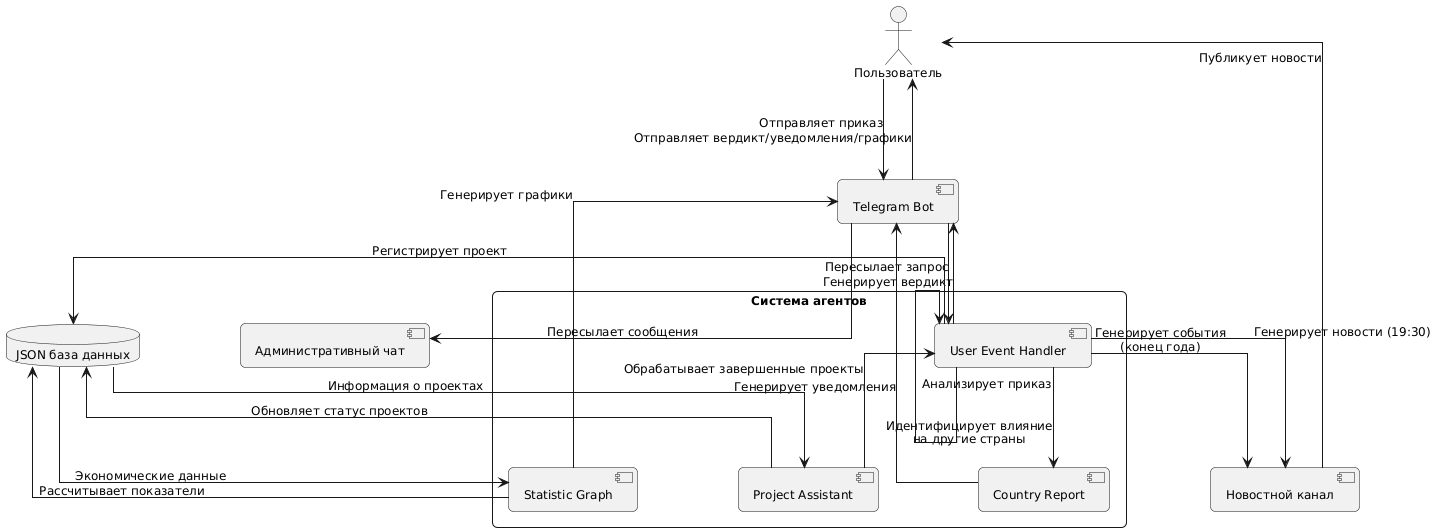
\includegraphics[width=\textwidth]{figures/agents.png}
    \caption{Основные компоненты системы и их взаимодействие}
    \label{fig:agents}
\end{figure}\\
\subsubsection{Ограничения прототипа}

Для первичного прототипа были приняты следующие сознательные ограничения:

\begin{itemize}
    \item \textbf{Ограниченное количество игроков} — прототип был рассчитан на участие 9 игроков, что позволяло обеспечить комфортную нагрузку на систему и внимательно отслеживать процесс тестирования.

    \item \textbf{Фиксированный сеттинг} — в отличие от некоторых ВПИ с процедурно генерируемым миром, RELOAD WPG использовал заранее определённый научно-фантастический сеттинг, основанный на вселенной оригинальной "{}Внеземной ВПИ"{}.

    \item \textbf{Упрощённая экономическая модель} — для первого прототипа была использована базовая экономическая система, не включающая детальное моделирование торговых отношений, ресурсных цепочек и сложных финансовых механизмов.

    \item \textbf{Зависимость от внешних API} — система использовала облачный API OpenAI для доступа к GPT-4, что накладывало ограничения на скорость обработки запросов и стоимость эксплуатации.
\end{itemize}

Таким образом, первичный прототип RELOAD WPG был спроектирован как целенаправленный эксперимент, призванный проверить жизнеспособность концепции автоматизированного вердерства с использованием языковых моделей и сформировать основу для более совершенной системы на основе полученного опыта и обратной связи пользователей.

\subsection{Интеграция с Telegram и выбор языковой модели}

Выбор платформы для реализации пользовательского интерфейса и интеграция с языковой моделью являлись критически важными аспектами разработки первичного прототипа, определяющими доступность, удобство использования и технические возможности системы. Для прототипа была выбрана комбинация мессенджера Telegram в качестве интерфейсной платформы и языковой модели GPT-4 от OpenAI в качестве основного генеративного компонента.

\subsubsection{Интеграция с Telegram}

Telegram был выбран в качестве платформы для разработки пользовательского интерфейса по ряду причин:

\begin{itemize}
    \item \textbf{Широкая распространённость} среди целевой аудитории ВПИ, подтверждённая результатами предварительного опроса потенциальных игроков.

    \item \textbf{Развитый Bot API}, предоставляющий необходимые инструменты для создания интерактивных ботов с поддержкой кнопок, форматированного текста и медиафайлов.

    \item \textbf{Экосистема каналов и групп}, позволяющая организовать разные аспекты игрового взаимодействия (личные сообщения, новостная лента, общий чат) в рамках единой платформы.

    \item \textbf{Кроссплатформенность}, обеспечивающая доступ к игре с различных устройств (мобильные телефоны, планшеты, компьютеры) без необходимости разработки отдельных клиентских приложений.
\end{itemize}

Архитектура интеграции с Telegram включала следующие компоненты:

\begin{enumerate}
    \item \textbf{Основной игровой бот} (@reload\_wpg\_bot) — центральный элемент взаимодействия, через который игроки отправляли приказы, получали вердикты и управляли своими государствами.

    \item \textbf{Новостной канал} (@reload\_wpg\_news) — публичный канал для распространения информации о ключевых событиях в игровом мире, правилах и обновлениях системы.

    \item \textbf{Общий чат} (@reload\_wpg\_chat) — групповой чат для общения между участниками, обсуждения игровых событий и неформального взаимодействия.
\end{enumerate}

Пользовательский интерфейс бота был спроектирован с учётом специфики текстовых стратегических игр и включал следующие ключевые элементы:

\begin{itemize}
    \item \textbf{Процесс регистрации и онбординга} — при первом запуске бота пользователю предлагалось пройти короткую процедуру инициализации, включающую выбор страны из 9 доступных (соответствующих государствам из оригинальной "{}Внеземной ВПИ"{}) и выбор уровня подписки (от бесплатного до премиум).

    \item \textbf{Клавиатура с основными функциями} — постоянно доступный набор кнопок, включающий доступ к карте, графикам, проектам, информации о стране, настройкам погружения и функции отправки телеграмм другим игрокам.

    \item \textbf{Текстовый ввод} — основной метод взаимодействия, позволяющий игрокам формулировать приказы, задавать вопросы и инициировать проекты в свободной форме, без необходимости следования строгим синтаксическим правилам.
\end{itemize}

Одной из технических особенностей реализации стало создание механизма, позволяющего администратору игры отправлять сообщения через бота от его имени, что обеспечивало возможность ручного вмешательства в процесс игры при необходимости корректировки генерируемого контента.

\subsubsection{Выбор и настройка языковой модели}

В качестве основы для генерации вердиктов и ответов на вопросы игроков была выбрана языковая модель GPT-4 от OpenAI, доступная через API. Этот выбор был обусловлен следующими факторами:

\begin{itemize}
    \item \textbf{Превосходное качество генерации} длинных связных текстов с сохранением контекста, что критически важно для создания вердиктов в жанре ВПИ.

    \item \textbf{Способность к условному рассуждению} и логической связности при генерации событий, обеспечивающая реалистичность и непротиворечивость игрового нарратива.

    \item \textbf{Гибкость в настройке} через систему промптов, позволяющая адаптировать модель к специфическим требованиям игрового контекста без необходимости дополнительного обучения.

    \item \textbf{Доступность через API} с предсказуемой моделью тарификации, что упрощало разработку и позволяло прогнозировать эксплуатационные расходы.
\end{itemize}

Для обеспечения оптимального функционирования модели в контексте ВПИ были применены следующие подходы к её настройке:

\begin{enumerate}
    \item \textbf{Разработка базового системного промпта}, определяющего общий контекст игры, сеттинг, технологические ограничения эпохи и ключевые механики взаимодействия.

    \item \textbf{Создание специализированных промптов} для различных типов агентов (обработчик событий, генератор отчётов о странах, ассистент проектов, статистический анализатор), оптимизирующих модель для выполнения конкретных функций.

    \item \textbf{Настройка параметра температуры} для обеспечения баланса между детерминированностью и творческим разнообразием. Для большинства операций использовалось значение temperature = 0.7, обеспечивающее достаточную вариативность при сохранении логической согласованности.

    \item \textbf{Экспериментальная валидация промптов} с использованием различных формулировок и структур для выявления наиболее эффективных подходов к инструктированию модели.
\end{enumerate}

В процессе тестирования прототипа, в ответ на рост эксплуатационных расходов, связанных с интенсивным использованием модели, особенно во время военных действий когда стоимость достигла \$10 в сутки, была осуществлена миграция на более экономичную модель GPT-4o mini. Примечательно, что, согласно отзывам игроков, это изменение не привело к заметному снижению качества генерируемых вердиктов, что свидетельствует о потенциальной возможности использования более компактных и эффективных моделей в будущих итерациях системы.

\subsubsection{Интерфейс взаимодействия и правила игры}

Для облегчения вхождения пользователей в игровой процесс были разработаны подробные правила и руководство по использованию бота, доступные через новостной канал. Основные положения включали:

\begin{itemize}
    \item \textbf{Общее описание} игры, её жанра, сеттинга и временной линии, начинающейся в 2650 году, за несколько лет до знакового события оригинальной ВПИ — Восьмидесятилетней войны.

    \item \textbf{Уровни погружения} — система подписок, определяющая доступные функции и частоту взаимодействия:
    \begin{itemize}
        \item Уровень 1 (бесплатный) — базовый доступ с ограниченной частотой приказов
        \item Уровень 2 (150 рублей в неделю) — дополнительные функции и повышенная частота взаимодействия
        \item Уровень 3 (450 рублей в неделю) — максимальные возможности, включая доступ к графикам и наиболее высокая частота взаимодействия
    \end{itemize}

    \item \textbf{Специальные правила} — важные оговорки, такие как возможность администратора вмешиваться в игру, приоритет вердиктов администратора над автоматически генерируемыми и даже толерантность к "{}prompt injection"{} в развлекательных целях.

    \item \textbf{Инструкция по использованию бота} — детальное описание доступных функций и способов взаимодействия, включая отправку приказов, просмотр карты, управление проектами, отправку телеграмм другим правителям и доступ к аналитическим графикам.
\end{itemize}

Система кнопок в интерфейсе бота предоставляла доступ к ключевым функциям:

\begin{itemize}
    \item \textbf{Карта} — визуальное представление мира с актуальными границами и контролируемыми территориями
    \item \textbf{Графики} — аналитические данные о динамике ВВП, лояльности и численности населения (доступны с III уровня погружения)
    \item \textbf{Проекты} — список активных долгосрочных инициатив и их статус готовности
    \item \textbf{Страна} — информация о текущем государстве игрока и возможность смены страны (функция находилась в разработке)
    \item \textbf{Телеграмма} — функция отправки сообщений правителям других стран (доступна со II уровня погружения)
    \item \textbf{Погружение} — управление уровнем подписки и соответствующими возможностями
\end{itemize}

Реализованный интерфейс обеспечивал баланс между удобством использования и функциональностью, однако уже на этапе первичного тестирования выявились определённые недостатки, такие как недостаточная заметность ссылки на новостной канал в приветственном сообщении, что потребовало дополнительных коммуникаций с игроками. Эти наблюдения стали важной частью обратной связи для планирования улучшений интерфейса в последующих версиях системы.

\subsection{Система агентов и обработка приказов}

Ядром функциональности первичного прототипа RELOAD WPG являлась система специализированных агентов, отвечающих за обработку пользовательских запросов и поддержание согласованного состояния игрового мира. Архитектура системы была построена по принципу разделения ответственности, где каждый агент выполнял определённую функцию в цепочке обработки информации.

\subsubsection{Архитектура системы агентов}

Система включала четыре основных агента, взаимодействующих между собой и с хранилищем данных:

\begin{enumerate}
    \item \textbf{User Event Handler (Обработчик пользовательских событий)} — центральный агент, принимающий входящие сообщения от пользователей, классифицирующий их и определяющий дальнейший маршрут обработки. Этот агент выполнял следующие ключевые функции:
    \begin{itemize}
        \item Определение типа сообщения (приказ, вопрос, запрос информации)
        \item Анализ приказа для выявления стран, на которые он может оказать влияние
        \item Идентификация долгосрочных проектов и оценка времени их выполнения
        \item Генерация случайных событий в конце игрового года
        \item Формирование структурированного JSON-представления обработанного приказа для дальнейшего использования другими агентами
        \item Генерация ежедневных новостей, которые публиковались в новостном канале в 19:30
    \end{itemize}

    \item \textbf{Country Report (Отчёт о стране)} — агент, отвечающий за генерацию уведомлений о влиянии действий одного государства на другие. Активировался в следующих случаях:
    \begin{itemize}
        \item Когда страна явно упоминалась в приказе или вердикте другого игрока
        \item Когда действие одного государства косвенно затрагивало интересы другого государства (с определённой вероятностью)
        \item При генерации реакций на значимые международные события
    \end{itemize}

    \item \textbf{Project Assistant (Ассистент проектов)} — агент, управляющий жизненным циклом долгосрочных проектов. Его функции включали:
    \begin{itemize}
        \item Отслеживание статуса выполнения проектов
        \item Генерацию итоговых отчётов по завершённым проектам в конце игрового года
        \item Обновление информации о проектах в базе данных
    \end{itemize}

    \item \textbf{Statistic Graph (Статистический график)} — агент, отвечающий за экономические и демографические расчёты. Функционал включал:
    \begin{itemize}
        \item Анализ экономического влияния действий игрока на основе информации из треда
        \item Расчёт изменений ВВП, лояльности и численности населения в конце игрового года
        \item Формирование данных для визуализации динамики ключевых показателей в виде графиков
        \item Хранение и обновление экономических показателей в базе данных
    \end{itemize}
\end{enumerate}

\subsubsection{Хранение и управление данными}

Для хранения игрового состояния была реализована простая, но эффективная система на основе JSON-файлов:

\begin{itemize}
    \item \textbf{Базовые данные о странах} — каждое государство имело связанную запись, содержащую основную информацию:
    \begin{itemize}
        \item Название и идентификатор
        \item Текущие значения ВВП, лояльности и численности населения
        \item Историю изменения этих показателей для построения графиков
    \end{itemize}

    \item \textbf{Журнал проектов} — структурированный список активных и завершённых проектов с атрибутами:
    \begin{itemize}
        \item Название и описание проекта
        \item Игрок-инициатор
        \item Год начала и ожидаемый год завершения
        \item Статус проекта
    \end{itemize}
\end{itemize}

История взаимодействий с пользователями сохранялась непосредственно в Telegram-чатах и дублировалась в административную беседу, куда пересылались все сообщения игроков и ответы системы. Это обеспечивало возможность мониторинга игрового процесса администраторами и служило дополнительным резервным хранилищем истории взаимодействий.

\subsubsection{Процесс обработки приказов}

Типичный жизненный цикл обработки приказа игрока включал следующую последовательность шагов:

\begin{enumerate}
    \item \textbf{Приём сообщения} — пользователь отправлял текстовый приказ через интерфейс Telegram-бота.

    \item \textbf{Первичный анализ} — User Event Handler анализировал сообщение с помощью GPT-4 для определения его типа, выявления затрагиваемых стран и идентификации возможных проектов.

    \item \textbf{Генерация вердикта} — на основе приказа и контекстной информации о текущем состоянии страны формировался запрос к GPT-4 для генерации вердикта, описывающего результаты выполнения приказа.

    \item \textbf{Отправка ответа пользователю} — сгенерированный вердикт отправлялся игроку через бота.

    \item \textbf{Обработка межгосударственного влияния} — если приказ затрагивал интересы других стран, Country Report генерировал соответствующие уведомления и отправлял их заинтересованным игрокам.

    \item \textbf{Регистрация проектов} — если приказ инициировал долгосрочный проект, информация о нём фиксировалась в базе данных с указанием ожидаемого срока завершения.

    \item \textbf{Обновление игрового состояния} — по итогам обработки приказа могли обновляться различные аспекты игрового состояния, включая экономические показатели.
\end{enumerate}

В конце каждого игрового года (который соответствовал нескольким дням реального времени) происходили дополнительные процессы:

\begin{itemize}
    \item Project Assistant проверял список проектов, выявлял завершённые в текущем году и генерировал итоговые отчёты по ним.

    \item Statistic Graph анализировал экономическое влияние всех действий за год и рассчитывал обновлённые значения ВВП, лояльности и численности населения.

    \item User Event Handler генерировал случайные события для каждой страны, добавляя элемент непредсказуемости и динамики в игровой процесс.
\end{itemize}

Кроме того, User Event Handler ежедневно в 19:30 генерировал и публиковал в новостном канале сводку основных событий, произошедших в игровом мире. Эти новости служили важным элементом формирования общей картины происходящего для всех игроков и способствовали созданию единого информационного пространства.

\subsubsection{Проблемы и ограничения первичной архитектуры}

В ходе тестирования прототипа были выявлены несколько ключевых ограничений выбранной архитектуры:

\begin{itemize}
    \item \textbf{Ограниченная контекстуальная память} — поскольку каждый запрос к GPT-4 обрабатывался независимо, система сталкивалась с трудностями в поддержании долгосрочной согласованности и запоминании специфических деталей игрового мира, не включённых явно в контекст запроса.

    \item \textbf{Проблемы с межгосударственным взаимодействием} — изначальная реализация, где каждый игрок имел отдельный "{}тред"{} для взаимодействия, приводила к изоляции действий игроков друг от друга. Это ограничение было частично преодолено путём объединения всех игроков в общий тред, однако генерация уведомлений о влиянии действий других стран часто воспринималась игроками как навязчивая и нереалистичная.

    \item \textbf{Нереалистичные временные оценки проектов} — языковая модель имела тенденцию назначать необоснованно длительные сроки даже для относительно простых проектов (например, "{}отправка послов"{} могла оцениваться в 10-15 лет), что негативно влияло на динамику игры и вызывало фрустрацию у игроков.

    \item \textbf{Галлюцинации и несогласованность} — модель иногда генерировала фактически неверную информацию или противоречила ранее установленным фактам, особенно при взаимодействии нескольких игроков в одном контексте.

    \item \textbf{Высокая стоимость эксплуатации} — интенсивное использование API GPT-4, особенно в периоды активных военных действий, приводило к значительным эксплуатационным расходам (до \$10 в сутки), что ставило под вопрос экономическую устойчивость выбранного подхода в долгосрочной перспективе.
\end{itemize}

Для адаптации к выявленным ограничениям в ходе игровой сессии были внедрены несколько тактических улучшений:

\begin{itemize}
    \item Введение "{}боевого режима"{}, позволяющего обрабатывать военные приказы с минимальными задержками, минуя стандартный механизм проектов.

    \item Настройка вероятностных параметров для уведомлений о межгосударственном влиянии (50\% при явном упоминании страны и 5\% в иных случаях), что снизило частоту нерелевантных уведомлений.

    \item Оптимизация использования контекстного окна для включения наиболее релевантной исторической информации при генерации вердиктов.

    \item Переход на более экономичную модель GPT-4o mini для снижения эксплуатационных расходов, что, неожиданно, не привело к заметному снижению качества вердиктов по отзывам игроков.
\end{itemize}

Опыт разработки и тестирования первичной системы агентов и механизмов обработки приказов предоставил ценную информацию для проектирования улучшенной архитектуры в последующих версиях, с акцентом на более эффективное управление контекстом, реалистичное моделирование темпоральных аспектов игрового мира и экономичное использование языковых моделей.

\subsection{Механизмы проектов и межгосударственного взаимодействия}

Для обеспечения глубины и динамики игрового процесса в RELOAD WPG были реализованы два ключевых механизма: система долгосрочных проектов и различные каналы межгосударственного взаимодействия. Эти компоненты играли центральную роль в создании ощущения прогресса и связности игрового мира, а также стимулировали социальную составляющую игры.

\subsubsection{Система долгосрочных проектов}

Механизм проектов был разработан для моделирования масштабных долгосрочных инициатив, требующих значительного времени для реализации. Этот механизм позволял игрокам планировать стратегическое развитие своих государств, а не ограничиваться только тактическими решениями с немедленным эффектом.

\paragraph{Структура и хранение данных о проектах}

Информация о проектах хранилась в структурированном формате JSON, что обеспечивало удобство обработки и обновления данных. Для каждого проекта фиксировались следующие ключевые параметры:

\begin{itemize}
    \item \textbf{Название и краткое описание} — идентификаторы проекта в системе
    \item \textbf{Игрок-инициатор} — государство, начавшее проект
    \item \textbf{Год начала} — дата запуска проекта в игровом времени
    \item \textbf{Ожидаемый год завершения} — прогнозируемая дата завершения проекта
    \item \textbf{Статус} — текущее состояние проекта (активный, завершённый)
\end{itemize}

Пример структуры JSON для хранения проекта:

\begin{verbatim}
{
  "{}project_id"{}: "{}LRK-0023"{},
  "{}name"{}: "{}Космодром на острове Кэй"{},
  "{}description"{}: "{}Строительство космического порта для запуска орбитальных шаттлов"{},
  "{}initiator"{}: "{}Республика Лурк"{},
  "{}start_year"{}: 2655,
  "{}estimated_completion_year"{}: 2662,
  "{}status"{}: "{}active"{}
}
\end{verbatim}

\paragraph{Жизненный цикл проекта}

Процесс создания и реализации проектов включал следующие этапы:

\begin{enumerate}
    \item \textbf{Инициация} — игрок формулировал инициативу в форме текстового приказа. User Event Handler анализировал приказ и определял, является ли он долгосрочным проектом, требующим отложенного результата.

    \item \textbf{Оценка сроков} — система автоматически определяла ожидаемое время выполнения проекта, основываясь на его масштабе, технологической сложности и соответствии текущему уровню развития государства. На этом этапе возникла одна из наиболее заметных проблем прототипа: языковая модель имела тенденцию устанавливать необоснованно длительные сроки даже для относительно простых проектов.

    \item \textbf{Регистрация} — после определения параметров проект фиксировался в базе данных со статусом "{}активный"{}.

    \item \textbf{Мониторинг} — игроки могли просматривать список своих активных проектов через интерфейс бота, используя кнопку "{}Проекты"{}. Это обеспечивало прозрачность процесса и позволяло отслеживать прогресс.

    \item \textbf{Завершение} — когда наступал год завершения проекта, Project Assistant генерировал отчёт о результатах и последствиях реализации инициативы. Этот отчёт учитывал как изначальные параметры проекта, так и изменения в игровом мире, произошедшие за время его выполнения.
\end{enumerate}

\paragraph{Выявленные проблемы и адаптации}

В ходе тестирования прототипа были выявлены несколько ключевых проблем, связанных с системой проектов:

\begin{itemize}
    \item \textbf{Нереалистичные временные оценки} — как упоминалось ранее, модель часто назначала чрезмерно длительные сроки выполнения. Приказы вроде "{}отправить послов"{} или "{}провести разведку"{} могли получать оценку в 10-15 лет, что вызывало фрустрацию у игроков и нарушало ощущение реалистичности.

    \item \textbf{Отсутствие промежуточных результатов} — первоначальная реализация не предусматривала получения промежуточных отчётов о ходе выполнения проектов, что снижало вовлечённость игроков в долгосрочные инициативы.

    \item \textbf{Ограниченная интеграция с общим контекстом} — некоторые проекты, особенно связанные с технологическим развитием, недостаточно интегрировались в общую картину мира и не влияли на другие аспекты игры, как отмечали игроки в обратной связи.
\end{itemize}

Для адаптации к этим ограничениям в ходе игровой сессии были внедрены следующие улучшения:

\begin{itemize}
    \item \textbf{Введение "{}боевого режима"{}} — специальный режим для военных операций, позволяющий обрабатывать приказы в ускоренном темпе, минуя стандартный механизм проектов. Это обеспечило более динамичное ведение военных действий.

    \item \textbf{Ручная корректировка сроков} — в случаях, когда оценка временем выполнения была явно нереалистичной, администратор вмешивался и корректировал параметры проекта.

    \item \textbf{Упрощение многозадачности} — для игроков с базовым уровнем подписки была добавлена возможность включать несколько приказов в одно сообщение (как отдельные абзацы), что позволило им эффективнее управлять своими государствами несмотря на ограничения по частоте взаимодействия.
\end{itemize}

\subsubsection{Механизмы межгосударственного взаимодействия}

Взаимодействие между государствами является фундаментальным аспектом жанра ВПИ, требующим эффективных каналов коммуникации и инструментов влияния. В рамках прототипа были реализованы несколько механизмов для обеспечения такого взаимодействия.

\paragraph{Каналы коммуникации}

Игроки RELOAD WPG имели доступ к нескольким каналам для взаимодействия:

\begin{itemize}
    \item \textbf{Система телеграмм} — встроенная в бота функция отправки официальных сообщений другим правителям. Доступ к этой функции предоставлялся начиная со второго уровня подписки и использовался для формальной дипломатической коммуникации.

    \item \textbf{Общий чат} (@reload\_wpg\_chat) — групповой Telegram-чат для всех участников игры, где происходило неформальное обсуждение игровых событий, обмен мнениями и публичная дипломатия.

    \item \textbf{Личные сообщения} — игроки активно использовали прямую коммуникацию через Telegram для ведения тайных переговоров, заключения альянсов и координации совместных действий, что добавляло игре глубину и стратегическое измерение.
\end{itemize}

Такое разнообразие каналов позволяло игрокам выбирать наиболее подходящий формат коммуникации в зависимости от ситуации — от публичных деклараций до секретных договорённостей.

\paragraph{Система влияния действий на другие государства}

Для моделирования взаимозависимости государств в игровом мире была разработана система автоматического оповещения о влиянии действий одной страны на другие. Эта система функционировала следующим образом:

\begin{enumerate}
    \item User Event Handler анализировал каждый приказ для выявления потенциального влияния на другие государства.

    \item Если в приказе или вердикте явно упоминалось название другого государства, Country Report генерировал соответствующее уведомление с вероятностью 50\%.

    \item Даже без явного упоминания система могла определить косвенное влияние действий на другие страны и сгенерировать уведомление с вероятностью 5\%.

    \item Сгенерированное уведомление отправлялось затронутым игрокам, информируя их о действиях соседа и потенциальном влиянии на их государство.
\end{enumerate}

Пример такого уведомления:

\begin{verbatim}
🔍 Внешнеполитическая разведка Республики Лурк доносит:

Империя Хуан-Фернандес начала масштабную модернизацию своего флота,
уделяя особое внимание дредноутам дальнего действия. Аналитики отмечают,
что новые корабли оснащены усовершенствованными орудиями, способными
поражать цели на значительном расстоянии, включая территориальные воды Лурка.

Министерство обороны рекомендует усилить патрулирование прибрежных зон
и рассмотреть возможность модернизации собственных оборонительных систем.
\end{verbatim}

\paragraph{Проблемы и решения}

Реализация системы межгосударственного взаимодействия выявила ряд проблем:

\begin{itemize}
    \item \textbf{Изоляция действий игроков} — в начальной версии прототипа каждый игрок имел собственный изолированный "{}тред"{} взаимодействия с моделью, что приводило к ситуации, когда действия одного игрока никак не влияли на других. Система просто не знала о действиях других участников.

    \item \textbf{Навязчивые уведомления} — после введения системы влияния действий игроки начали получать слишком много уведомлений, многие из которых воспринимались как нерелевантные. Особенно распространённым был шаблон вида "{}Лурк выражает глубокую озабоченность действиями Хуан-Фернандеса"{}, ставший локальным мемом среди участников.

    \item \textbf{Несогласованность информации} — иногда разные игроки получали противоречивую информацию об одном и том же событии, что нарушало целостность игрового мира.
\end{itemize}

Для решения этих проблем были предприняты следующие меры:

\begin{itemize}
    \item \textbf{Объединение всех игроков в общий тред} — это позволило модели "{}видеть"{} действия всех участников и более корректно моделировать их взаимное влияние.

    \item \textbf{Настройка вероятностных параметров} для уведомлений: 50\% при явном упоминании страны и 5\% при косвенном влиянии. Это существенно снизило количество нерелевантных уведомлений.

    \item \textbf{Улучшение новостной ленты} — ежедневные новости стали важным инструментом создания единого информационного пространства, где освещались ключевые события, затрагивающие все государства.
\end{itemize}

\subsubsection{Эффективность и результаты}

Несмотря на выявленные проблемы, механизмы проектов и межгосударственного взаимодействия успешно выполнили свою роль в формировании комплексного и вовлекающего игрового опыта:

\begin{itemize}
    \item Система проектов позволила моделировать долгосрочное развитие государств, создавая ощущение прогресса и стратегической глубины.

    \item Разнообразные каналы коммуникации стимулировали активное взаимодействие между игроками, формирование альянсов и развитие сложных дипломатических отношений.

    \item Механизм уведомлений о влиянии действий, несмотря на первоначальные проблемы, после настройки обеспечил необходимую взаимозависимость государств в игровом мире.

    \item Сочетание формальных (через бота) и неформальных (в личных сообщениях) каналов взаимодействия обогатило игровой процесс, добавив элементы тайной дипломатии и интриг.
\end{itemize}

Опыт разработки и тестирования этих механизмов предоставил ценную информацию для проектирования улучшенной версии системы, с особым фокусом на более реалистичном моделировании временных аспектов проектов и более глубокой интеграции действий различных игроков в единый согласованный нарратив.

\subsection{Анализ обратной связи от игроков}

По завершении тестовой игровой сессии было проведено подробное исследование мнений участников с целью выявления сильных и слабых сторон прототипа, а также формирования требований к улучшенной версии системы. Сбор обратной связи осуществлялся через структурированную гугл-форму, включавшую как количественные оценки различных аспектов игры, так и качественные комментарии, позволившие глубже понять опыт пользователей.

\subsubsection{Методология сбора и структура обратной связи}

Для обеспечения комплексной оценки игрового опыта форма обратной связи была разделена на несколько тематических блоков:

\begin{itemize}
    \item \textbf{Общие впечатления от игры} — оценка общего уровня удовлетворенности
    \item \textbf{Оформление и визуальные аспекты} — включая дизайн бота, чата, новостного канала и карты
    \item \textbf{Функциональность бота} — оценка работы ключевых игровых механик
    \item \textbf{Игровой процесс} — включая баланс, динамику и сюжет
    \item \textbf{Открытые вопросы} — для получения развернутых мнений и предложений
\end{itemize}

Для количественной оценки использовалась 10-балльная шкала, где 1 соответствовала крайне негативной оценке, а 10 — максимально позитивной. Дополнительно игрокам предлагалось предоставить развернутые текстовые ответы на вопросы о наиболее понравившихся и разочаровавших аспектах игры, а также пожелания для будущих ВПИ.

\subsubsection{Количественные результаты оценки}

Анализ количественных оценок различных аспектов игры выявил следующую картину (приведены средние значения по 10-балльной шкале):

\begin{table}[h]
\centering
\begin{tabular}{|l|c|}
\hline
\textbf{Аспект игры} & \textbf{Средняя оценка} \\
\hline
Общие впечатления от игры & 7,25 \\
\hline
\multicolumn{2}{|l|}{\textit{Визуальное оформление}} \\
\hline
Оформление игры в целом & 7,63 \\
Оформление трейлера & 7,63 \\
Оформление тг-бота & 8,25 \\
Оформление чата & 7,38 \\
Оформление канала новостей & 7,38 \\
Оформление канала новостей & 7,38 \\
Оформление карты & 8,75 \\
\hline
\multicolumn{2}{|l|}{\textit{Функциональность бота}} \\
\hline
Впечатления от бота в целом & 5,63 \\
Ответы бота на вопросы & 5,00 \\
Оценка времени проектов & 5,13 \\
Ответы бота на приказы & 5,75 \\
Ассистент влияния на страны & 5,63 \\
Функционал бота & 5,25 \\
\hline
\multicolumn{2}{|l|}{\textit{Игровой процесс}} \\
\hline
Влияние рандома & 6,50 \\
Соответствие рамкам эпохи & 2,50 \\
Боевка & 4,13 \\
Общение между игроками & 6,75 \\
Сюжет & 7,00 \\
\hline
\end{tabular}
\caption{Средние оценки различных аспектов игры}
\label{tab:feedback-ratings}
\end{table}

Анализ количественных данных позволяет выделить следующие ключевые наблюдения:

\begin{itemize}
    \item \textbf{Высокие оценки визуального оформления} — все аспекты визуального дизайна были оценены выше 7 баллов, с особенно высокими оценками для карты (8,75) и оформления бота (8,25), что свидетельствует об успешной реализации пользовательского интерфейса.

    \item \textbf{Средние оценки функциональности бота} — все аспекты, связанные с работой языковой модели и игровых механик, получили оценки в диапазоне 5-6 баллов, что указывает на наличие значительного пространства для улучшения.

    \item \textbf{Крайне низкая оценка соответствия рамкам эпохи} (2,50) — этот аспект является наиболее проблемным с точки зрения игроков, свидетельствуя о недостаточном контроле языковой модели за технологическим и историческим соответствием генерируемого контента.

    \item \textbf{Относительно высокие оценки сюжета} (7,00) и общения между игроками (6,75) — эти аспекты подчеркивают успех в создании вовлекающего нарратива и формировании активного социального взаимодействия, несмотря на технические ограничения.
\end{itemize}

\subsubsection{Качественный анализ комментариев}

Анализ развернутых комментариев игроков позволил выявить более детальную картину их впечатлений и сгруппировать обратную связь по ключевым тематическим блокам (подробные результаты представлены в Приложении~\ref{appendix:2}).

\paragraph{Положительные аспекты}

Среди наиболее часто упоминаемых положительных сторон игры были выделены следующие:

\begin{itemize}
    \item \textbf{Концепция и общая система} — игроки отмечали потенциал идеи автоматизированного вердинга и общую привлекательность формата: \textit{"{}Концепция + в целом система крутая, хоть и требует доработок."{}}

    \item \textbf{Последовательность и возможность реализации уникальных идей} — способность системы поддерживать уникальный стиль игры за разные страны: \textit{"{}Неплохое consistency — ± получалось реализовать желаемые идеи, за счёт чего каждая страна действительно выглядела уникально."{}}

    \item \textbf{Реализация креативных концепций} — свобода в экспериментировании с нестандартными идеями: \textit{"{}Реализация самых безумных идей — это весело."{}}

    \item \textbf{Качество ролевого взаимодействия} — глубина и вовлеченность в социальные аспекты игры: \textit{"{}Отыгрыш (я получил огромное удовольствие от взаимодействия с другими игроками... У нас литералли был с A проект договора в пдфке с пунктами, так ещё и с посредником в переговорах)."{}}

    \item \textbf{Динамичный сюжет} — непредсказуемость и интересные повороты игрового нарратива: \textit{"{}Двигающие сюжет события, подкидываемые игрой."{}}

    \item \textbf{Аналитические инструменты} — положительные отзывы о графиках и статистике: \textit{"{}Графики! Их наличие действительно добавляет то дивное измерение игры, на которое можно фокусироваться."{}}
\end{itemize}

\paragraph{Проблемные аспекты}

Анализ критических замечаний выявил следующие ключевые проблемы:

\begin{itemize}
    \item \textbf{Дисбаланс между игроками с разными тарифами} — ощущение несправедливости из-за разной скорости получения вердиктов: \textit{"{}Pay2win + нет одного источника правды + бот часто не присылал что-то что происходит с моей страной."{}}

    \item \textbf{Ограниченная контекстуальная память} — недостаточное "{}запоминание"{} и использование ранее установленных фактов: \textit{"{}Периодически возникало ощущение neural mess... модельки, которая реагирует больше на то, как я оформлю приказ, чем на то, что было раньше."{}}

    \item \textbf{Потеря связности игрового мира} — недостаточная интеграция индивидуальных сюжетных линий в единый мир: \textit{"{}Из-за этого же — часть идей так и не удалось нормально реализовать, и они улетели в труху. Союз Пара, премия Золотой Гой, дирижабль с жабками, в принципе развитие аэротранспорта — бот реализовывал все это в рамках приказа, но дальше об этом никак не вспоминалось..."{}}

    \item \textbf{Галлюцинации и противоречия} — генерация фактически неверной информации: \textit{"{}Рандом, галлюцинирующий гпт"{}} и \textit{"{}Бот очень сильно тупит, Хуан-Фернандес воюет с ХФ и Мордор требует капитуляцию ТСГЕМ это конечно смешно, но погружение портит."{}}

    \item \textbf{Отсутствие постепенного влияния на культуру} — невозможность плавных изменений игрового мира: \textit{"{}Все проблемы так или иначе будут про отсутствие воспринимаемой связности. ВПИ — это одна из тех штук, где взмах крыла бабочки вызывает ураганы. При игре с нейроботом это невозможно, пока не начинается что-то совсем шизофреническое. То есть, я не могу слегка изменять свою культуру."{}}

    \item \textbf{Нелогичная оценка сложности задач} — нереалистичные временные рамки для проектов разной сложности: \textit{"{}Очень странная разбалансировка сложностей приказов. Задачи в духе 'Последить за Мордором', 'Написать мафиози из ФТК' занимали больше времени, чем 'Разработать систему нейроинтерфейсов для слияния всех мыслей всех людей'."{}}

    \item \textbf{Слишком быстрый технологический прогресс} — недостаточный контроль за темпами развития: \textit{"{}Что из-за gpt может произойти вообще что угодно. Прогресс несся быстрее, чем успевали следить. Вот только что были дирижабли, проходит неделя и на меня нацеливают орбитальные пушки."{}}
\end{itemize}

\paragraph{Пожелания для будущих версий}

Игроки также предложили ряд идей и пожеланий для будущих версий системы:

\begin{itemize}
    \item \textbf{Улучшенный контроль за хронологией и технологической эпохой}: \textit{"{}Чтобы нейронка выдавала одинаковые ответы на одинаковые вопросы от разных игроков об одном и том же событии. Так же нейронка должна как-то помнить хронологию событий."{}}

    \item \textbf{Более насыщенная информационная среда}: \textit{"{}Больше вестей из других стран — иногда прямо информационный вакуум был."{}}

    \item \textbf{Более развитые механики взаимодействия между странами}: \textit{"{}Маловато в целом механик для взаимодействия с другими странами. С кем я торгую, на кого я могу так влиять, от кого я завишу, с кем у нас есть культурные связи итд."{}}

    \item \textbf{Баланс между автоматизацией и человеческим контролем}: \textit{"{}Вероятно, пока что нужно прикладывать чуть больше мясного мешка. Бот неплохо зарекомендовал себя как справочно-вопросная система, но, кажется, должен существовать ещё некий отсек 'Дизайна того, как выглядит игровой мир в целом вот прямо сейчас и что в нём важно', которым должен заниматься человек."{}}

    \item \textbf{Персонализированное внимание}: \textit{"{}В идеале личный верд."{}} — указание на желание более персонализированного и глубокого взаимодействия.

    \item \textbf{Более глубокая игровая механика}: \textit{"{}Что-то более похожее на ВПИ, а не на калькулятор с прикрученным флейвор-текстом, который сам не понимает что описывает."{}} — пожелание более сложной и нюансированной игровой механики.
\end{itemize}

\subsubsection{Ключевые выводы для разработки улучшенной версии}

На основе комплексного анализа обратной связи были сформулированы следующие ключевые выводы и направления для совершенствования системы:

\begin{enumerate}
    \item \textbf{Необходимость улучшения контекстуальной памяти} — критически важно обеспечить более надежное сохранение и использование ранее установленных фактов о мире и действиях игроков. Реализация эффективной RAG-системы для извлечения релевантного контекста представляется приоритетным направлением развития.

    \item \textbf{Усиление контроля за технологической эволюцией} — необходимо разработать механизмы, обеспечивающие реалистичные темпы и последовательность технологического прогресса, соответствующие установленным рамкам эпохи.

    \item \textbf{Балансировка временных оценок проектов} — требуется более реалистичная система определения сроков выполнения инициатив, учитывающая их сложность, масштаб и соответствие текущему технологическому уровню.

    \item \textbf{Улучшение боевой системы} — учитывая низкие оценки текущей реализации (4,13 из 10), необходимо разработать более стратегически глубокую и реалистичную систему моделирования военных конфликтов.

    \item \textbf{Обеспечение согласованности информации} — важно минимизировать противоречия и несогласованность в информации, предоставляемой разным игрокам об одних и тех же событиях.

    \item \textbf{Оптимизация экономической модели} — эффективное использование языковых моделей с меньшими вычислительными требованиями (как показал опыт перехода на GPT-4o mini) может снизить эксплуатационные расходы без существенной потери качества.

    \item \textbf{Поддержка развития социальных аспектов} — учитывая высокие оценки социального взаимодействия и сюжета, следует сохранить и усилить элементы, способствующие активному взаимодействию между игроками и формированию увлекательного нарратива.
\end{enumerate}

В целом, анализ обратной связи подтвердил жизнеспособность концепции автоматизированного вердинга с использованием языковых моделей, несмотря на выявленные технические ограничения первичного прототипа. Успех в создании вовлекающего игрового опыта, положительные оценки общих впечатлений (7,25 из 10) и качественные отзывы о творческих аспектах свидетельствуют о потенциале данного подхода при условии решения выявленных проблем в последующих итерациях.

\subsection{Выявленные проблемы и ключевые выводы}

Проведение тестовой игровой сессии с использованием первичного прототипа RELOAD WPG и последующий анализ обратной связи от участников позволили выявить ряд существенных проблем и сформулировать ключевые выводы, имеющие важное значение как для оценки успешности прототипа, так и для определения направлений дальнейшего развития проекта.

\subsubsection{Систематизация выявленных проблем}

Выявленные в ходе тестирования проблемы можно систематизировать по нескольким ключевым категориям:

\paragraph{Проблемы контекстуальной памяти и согласованности}

Одной из наиболее критичных проблем оказалась ограниченная способность системы поддерживать долгосрочную согласованность игрового мира:

\begin{itemize}
    \item \textbf{Потеря контекста между взаимодействиями} — языковая модель не всегда эффективно "{}запоминала"{} ранее установленные факты, особенно если они не входили явно в контекст текущего запроса. Игроки описывали это как ощущение "{}neural mess"{}, когда модель больше реагировала на формулировку приказа, чем на предыдущую историю взаимодействия.

    \item \textbf{Взаимная изоляция игровых линий} — инициативы и проекты, начатые отдельными игроками, часто не интегрировались в общую картину мира и оставались изолированными в рамках индивидуальных сюжетных линий, что подрывало ощущение единого игрового пространства.

    \item \textbf{Противоречивая информация} — разные игроки могли получать несогласованную информацию об одних и тех же событиях, что нарушало логическую целостность игрового мира.

    \item \textbf{Галлюцинации и фактические ошибки} — модель периодически генерировала ошибочную информацию или создавала логические противоречия, например, "{}Хуан-Фернандес воюет с ХФ"{} (страна воюет сама с собой) или "{}Мордор требует капитуляцию ТСГЕМ"{} (членом которого сам являлся).
\end{itemize}

\paragraph{Проблемы балансировки игрового процесса}

Тестирование выявило ряд проблем, связанных с балансом и динамикой игрового процесса:

\begin{itemize}
    \item \textbf{Нереалистичные временные оценки проектов} — система часто назначала необоснованно длительные сроки для относительно простых проектов (10-15 лет на отправку послов) и одновременно недооценивала сложность масштабных технологических инноваций.

    \item \textbf{Несоответствие рамкам эпохи} — крайне низкая оценка данного аспекта игроками (2,5 из 10) отражала проблему неконтролируемого технологического прогресса и смешения технологий разных исторических периодов.

    \item \textbf{Дисбаланс между игроками с разными тарифами} — игроки с базовым уровнем подписки испытывали ощущение несправедливости из-за разной скорости получения вердиктов, характеризуя ситуацию как "{}pay-to-win"{}.

    \item \textbf{Недостаточная глубина боевой системы} — моделирование военных конфликтов получило относительно низкую оценку (4,13 из 10), что указывало на необходимость более стратегически глубокого подхода к этому аспекту игры.
\end{itemize}

\paragraph{Технические и экономические ограничения}

Разработка и эксплуатация прототипа выявили ряд технических и экономических вызовов:

\begin{itemize}
    \item \textbf{Высокая стоимость API-запросов} — интенсивное использование API GPT-4, особенно в периоды активных военных действий, приводило к значительным эксплуатационным расходам (до \$10 в сутки).

    \item \textbf{Ограничения контекстного окна} — даже при использовании моделей с большим контекстным окном сохранялись проблемы с эффективной передачей всей необходимой предыстории в контексте запросов.

    \item \textbf{Сложность настройки оптимальных промптов} — поиск баланса между детализацией инструкций и эффективным использованием контекстного пространства представлял нетривиальную задачу.

    \item \textbf{Навязчивые уведомления о межгосударственном влиянии} — первоначальная реализация механизма уведомлений часто генерировала нерелевантные сообщения, ставшие источником мемов среди игроков ("{}Лурк выражает глубокую озабоченность..."{}).
\end{itemize}

\subsubsection{Примененные решения и их эффективность}

В ходе тестовой игровой сессии был реализован ряд адаптивных решений, направленных на преодоление выявленных проблем:

\begin{itemize}
    \item \textbf{Объединение игроков в общий тред} — для решения проблемы изоляции действий игроков был осуществлен переход от индивидуальных тредов к общему контексту, что значительно улучшило взаимную интеграцию сюжетных линий.

    \item \textbf{Настройка вероятностных параметров уведомлений} — корректировка вероятности генерации уведомлений (50\% при явном упоминании страны и 5\% в иных случаях) существенно снизила проблему навязчивых и нерелевантных сообщений.

    \item \textbf{Введение "{}боевого режима"{}} — для повышения динамики военных действий был внедрен специальный режим, позволяющий обрабатывать приказы с минимальными задержками, минуя стандартный механизм проектов.

    \item \textbf{Возможность многозадачности для игроков первого уровня} — разрешение включать несколько приказов в одно сообщение для игроков с базовым тарифом частично смягчило проблему дисбаланса между разными уровнями подписки.

    \item \textbf{Переход на более экономичную модель} — миграция с GPT-4 на GPT-4o mini позволила существенно снизить эксплуатационные расходы без заметного (по отзывам игроков) снижения качества генерируемого контента.
\end{itemize}

Данные решения продемонстрировали разную степень эффективности, однако в целом позволили значительно улучшить игровой опыт в рамках тестовой сессии. Особенно успешными оказались объединение игроков в общий тред, оптимизация вероятностных параметров уведомлений и введение "{}боевого режима"{}, что нашло отражение в положительных отзывах игроков о динамике игрового процесса и увлекательности сюжета (7,0 из 10).

\subsubsection{Ключевые выводы}

На основе проведенного тестирования и анализа обратной связи можно сформулировать следующие ключевые выводы:

\begin{enumerate}
    \item \textbf{Принципиальная жизнеспособность концепции} — несмотря на выявленные ограничения, первичный прототип успешно подтвердил фундаментальную гипотезу о возможности использования языковых моделей для автоматизации роли вердера в ВПИ. Общая оценка игры участниками (7,25 из 10) свидетельствует о положительном восприятии концепции.

    \item \textbf{Критическая важность контекстуальной памяти} — для успешного функционирования подобной системы необходим эффективный механизм хранения, извлечения и использования информации о предыдущих событиях и установленных фактах игрового мира. Это направление должно стать приоритетным при разработке улучшенной версии.

    \item \textbf{Необходимость строгого контроля за технологической эволюцией} — для обеспечения достоверности и последовательности игрового мира критически важно разработать механизмы, ограничивающие неконтролируемый технологический прогресс и анахронизмы.

    \item \textbf{Потенциал экономической оптимизации} — опыт перехода на более экономичную модель GPT-4o mini без заметной потери качества указывает на возможность значительного снижения эксплуатационных расходов при правильной оптимизации системы.

    \item \textbf{Баланс между автоматизацией и человеческим контролем} — оптимальный подход к автоматизации вердерства предполагает сохранение определенной роли человека-администратора, особенно в вопросах поддержания согласованности игрового мира и разрешения сложных ситуаций.

    \item \textbf{Приоритетные направления улучшения} — на основе обратной связи можно выделить три ключевых направления для улучшения системы: 1) совершенствование механизмов поддержания контекстуальной памяти и согласованности, 2) разработка более реалистичной системы оценки времени выполнения проектов, 3) углубление боевой системы и других аспектов игровой механики.

    \item \textbf{Значение социальных аспектов} — высокие оценки взаимодействия между игроками (6,75 из 10) и увлекательность сюжета (7,0 из 10) подчеркивают важность социальной составляющей ВПИ и необходимость создания условий для активного взаимодействия и сотворчества участников.
\end{enumerate}

Подробное описание опыта разработки и результатов тестирования первичного прототипа было опубликовано автором в статье «RELOAD WPG: Первая нейроВПИ»~\cite{reload-article}. Исходный код прототипа доступен в открытом репозитории на GitHub~\cite{reload-github}, что позволяет заинтересованным исследователям и разработчикам изучить техническую реализацию описанных решений и использовать их в качестве основы для собственных проектов.

\subsubsection{Перспективы дальнейшего развития}

Опыт разработки и тестирования первичного прототипа предоставил ценную информацию для определения перспективных направлений дальнейшего развития проекта:

\begin{itemize}
    \item \textbf{Внедрение RAG-системы} для эффективного извлечения релевантной информации из базы знаний о игровом мире, что позволит значительно улучшить контекстуальную память и согласованность генерируемого контента.

    \item \textbf{Разработка специализированной боевой системы} с использованием внешних инструментов симуляции (например, Mesa или Ultimate Epic Battle Simulator) для создания более стратегически глубоких и визуально впечатляющих военных конфликтов.

    \item \textbf{Локальное развертывание языковых моделей} на предоставленной компанией МТС вычислительной инфраструктуре, что позволит существенно снизить эксплуатационные расходы и преодолеть ограничения, связанные с использованием облачных API.

    \item \textbf{Оптимизация архитектуры агентов} с более четким разделением ответственности и специализацией отдельных компонентов, что повысит общую надежность и предсказуемость системы.

    \item \textbf{Создание более глубокой экономической модели} с детальным моделированием торговых отношений, ресурсных зависимостей и других аспектов межгосударственного взаимодействия.
\end{itemize}

Эти направления составляют основу для разработки улучшенной версии системы, которая должна преодолеть ключевые ограничения первичного прототипа, сохранив при этом его успешные аспекты, такие как вовлекающий нарратив, активное социальное взаимодействие и творческая свобода.

В заключение можно отметить, что опыт разработки и тестирования RELOAD WPG как первой нейроВПИ не только подтвердил техническую возможность автоматизации вердерства с использованием языковых моделей, но и продемонстрировал потенциал такого подхода для расширения доступности и масштабов военно-политических игр. При этом выявленные проблемы и ограничения указывают на необходимость дальнейших исследований и технологических инноваций для полной реализации этого потенциала.